\documentclass[11pt,a4paper]{article}

\def\nyear {2025}
\def\nterm {Winter}
\def\nlecturer {}
\def\ncourse {Complex Analysis}

\makeatletter

% packages
\usepackage{amssymb,amsfonts,amsmath,calc,tikz,pgfplots,geometry,mathtools}
\usepackage{color}   % May be necessary if you want to color links
\usepackage[hidelinks]{hyperref}
\usepackage{forest}
\usepackage{commath} % ew
\usepackage{esdiff}
\usepackage{amsthm}
\usepackage{fancyhdr}
\usepackage{bm}
\usepackage{witharrows}
\usepackage{bookmark}
\usepackage{tikz-cd}
\usepackage{bbm}
\usepackage{textcomp}
\usepackage{gensymb}
\usepackage{cleveref}

% tikz libraries
\usetikzlibrary{positioning}
\usetikzlibrary{matrix}
\usetikzlibrary{arrows}
\usetikzlibrary{arrows.meta}
\usetikzlibrary{decorations.markings}

% Page style setup
\pagestyle{fancy}
\geometry{margin=1in}
\pgfplotsset{compat=1.18}
\setlength{\headheight}{14.6pt}
\addtolength{\topmargin}{-1.6pt}
\hypersetup{
    colorlinks=false,
    linktoc=section,
    linkcolor=black,
}

%% maketitle setup
\ifx \nauthor\undefined
  \def\nauthor{yehelip}
\else
\fi

\ifx \ncoursehead \undefined
\def\ncoursehead{\ncourse}
\fi

\lhead{\emph{\nouppercase{\leftmark}}}
\ifx \nextra \undefined
  \rhead{
    \ifnum\thepage=1
    \else
      \ncoursehead
    \fi}
\else
  \rhead{
    \ifnum\thepage=1
    \else
      \ncoursehead \ (\nextra)
    \fi}
\fi

\let\@real@maketitle\maketitle
\renewcommand{\maketitle}{\@real@maketitle\begin{center}
\begin{minipage}[c]{0.9\textwidth}\centering\footnotesize
These notes are not endorsed by the lecturers.
I have revised them outside lectures to incorporate supplementary explanations,
clarifications, and material for fun.
While I have strived for accuracy, any errors or misinterpretations 
are most likely mine.
\end{minipage}\end{center}}

% theorem environments
\theoremstyle{definition}
\newtheorem{definition}{Definition}[section]
\newtheorem{remark}{Remark}[section]
\newtheorem{example}{Example}[section]
\newtheorem{exercise}{Exercise}[section]
\newtheorem{paradox}{Paradox}[section]
\newtheorem*{solution}{Solution}
\theoremstyle{plain}
\newtheorem{theorem}{Theorem}[section]
\newtheorem{proposition}[theorem]{Proposition}
\newtheorem{lemma}[theorem]{Lemma}
\newtheorem{corollary}[theorem]{Corollary}

% tikz customization
\pgfarrowsdeclarecombine{twolatex'}{twolatex'}{latex'}{latex'}{latex'}{latex'}
\tikzset{->/.style = {decoration={markings,
                                  mark=at position 1
                                  with {\arrow[scale=2]{latex'}}},
                      postaction={decorate}}}
\tikzset{<-/.style = {decoration={markings,
                                  mark=at position 0 with {\arrowreversed[scale=2]{latex'}}},
                      postaction={decorate}}}
\tikzset{<->/.style = {decoration={markings,
                                   mark=at position 0 with {\arrowreversed[scale=2]{latex'}},
                                   mark=at position 1 with {\arrow[scale=2]{latex'}}},
                       postaction={decorate}}}
\tikzset{->-/.style = {decoration={markings,
                                   mark=at position #1 with {\arrow[scale=2]{latex'}}},
                       postaction={decorate}}}
\tikzset{-<-/.style = {decoration={markings,
                                   mark=at position #1 with {\arrowreversed[scale=2]{latex'}}},
                       postaction={decorate}}}
\tikzset{->>/.style = {decoration={markings,
                                  mark=at position 1 with {\arrow[scale=2]{latex'}}},
                      postaction={decorate}}}
\tikzset{<<-/.style = {decoration={markings,
                                  mark=at position 0 with {\arrowreversed[scale=2]{twolatex'}}},
                      postaction={decorate}}}
\tikzset{<<->>/.style = {decoration={markings,
                                   mark=at position 0 with {\arrowreversed[scale=2]{twolatex'}},
                                   mark=at position 1 with {\arrow[scale=2]{twolatex'}}},
                       postaction={decorate}}}
\tikzset{->>-/.style = {decoration={markings,
                                   mark=at position #1 with {\arrow[scale=2]{twolatex'}}},
                       postaction={decorate}}}
\tikzset{-<<-/.style = {decoration={markings,
                                   mark=at position #1 with {\arrowreversed[scale=2]{twolatex'}}},
                       postaction={decorate}}}

\pgfarrowsdeclare{biggertip}{biggertip}{%
  \setlength{\arrowsize}{1pt}
  \addtolength{\arrowsize}{.1\pgflinewidth}
  \pgfarrowsrightextend{0}
  \pgfarrowsleftextend{-5\arrowsize}
}{%
  \setlength{\arrowsize}{1pt}
  \addtolength{\arrowsize}{.1\pgflinewidth}
  \pgfpathmoveto{\pgfpoint{-5\arrowsize}{4\arrowsize}}
  \pgfpathlineto{\pgfpointorigin}
  \pgfpathlineto{\pgfpoint{-5\arrowsize}{-4\arrowsize}}
  \pgfusepathqstroke
}
\tikzset{
	EdgeStyle/.style = {>=biggertip}
}

\tikzset{circ/.style = {fill, circle, inner sep = 0, minimum size = 3}}
\tikzset{scirc/.style = {fill, circle, inner sep = 0, minimum size = 1.5}}
\tikzset{mstate/.style={circle, draw, black, text=black, minimum width=0.7cm}}

\tikzset{eqpic/.style={baseline={([yshift=-.5ex]current bounding box.center)}}}

\definecolor{mblue}{rgb}{0.2, 0.3, 0.8}
\definecolor{morange}{rgb}{1, 0.5, 0}
\definecolor{mgreen}{rgb}{0, 0.4, 0.2}
\definecolor{mred}{rgb}{0.5, 0, 0}

% topology
\newcommand{\Cells}{\text{Cells}}

% algebra
\DeclareMathOperator{\lcm}{lcm}
\DeclareMathOperator{\Out}{Out}
\DeclareMathOperator{\Aut}{Aut}
\DeclareMathOperator{\End}{End}
\DeclareMathOperator{\Inn}{Inn}
\DeclareMathOperator{\Mat}{Mat}
\DeclareMathOperator{\std}{std}
\DeclareMathOperator{\sgn}{sgn}
\DeclareMathOperator{\id}{id}
\DeclareMathOperator{\op}{op}
\DeclareMathOperator{\GL}{GL} % General linear group
\DeclareMathOperator{\SL}{SL} % Special linear group
\newcommand{\idealin}{\triangleleft}
\newcommand{\ip}[2]{\langle #1, #2 \rangle}
\newcommand{\bigslant}[2]
{{\raisebox{.2em}{$#1$}\left/\raisebox{-.2em}{$#2$}\right.}}

% analysis
\newcommand{\dx}{\dif x}
\newcommand{\dt}{\dif t}
\newcommand{\du}{\dif u}
\newcommand{\dv}{\dif v}
\newcommand{\dz}{\dif z}
\newcommand{\ds}{\dif s}
\newcommand{\dtheta}{\dif \theta}
\DeclareMathOperator{\im}{im}
\DeclareMathOperator{\cis}{cis}
\DeclareMathOperator{\Int}{Int}
\DeclareMathOperator{\diam}{diam}
\DeclareMathOperator{\supp}{supp}
\DeclareMathOperator{\Vol}{Vol} % Volume

% logic
\DeclareMathOperator{\MOD}{MOD}
\DeclareMathOperator{\Theory}{Theory}


% nice
\newcommand{\half}{\frac{1}{2}}
\newcommand{\pair}{\del}
\newcommand{\taking}[1]{\xrightarrow{#1}}
\newcommand{\inv}{^{-1}}
\newcommand{\ot}{\leftarrow}
\newcommand{\ninfty}{-\infty}
\newcommand{\floor}[1]{\left\lfloor #1 \right\rfloor}
\newcommand{\ceil}[1]{\left\lceil #1 \right\rceil}

% probability
\newcommand{\Prob}{\mathbf{P}}
\renewcommand{\vec}[1]{\boldsymbol{\mathbf{#1}}}
\DeclareMathOperator{\Bin}{Bin}
\DeclareMathOperator{\Geo}{Geo}
\DeclareMathOperator{\Poi}{Poi}
\DeclareMathOperator{\Exp}{Exp}
\DeclareMathOperator{\Var}{Var} % Variance
\DeclareMathOperator{\Cov}{Cov}

% special letters
\newcommand{\N}{\mathbb{N}}
\newcommand{\Z}{\mathbb{Z}}
\newcommand{\Q}{\mathbb{Q}}
\newcommand{\R}{\mathbb{R}}
\newcommand{\C}{\mathbb{C}}
\newcommand{\F}{\mathbb{F}}
\newcommand{\E}{\mathbb{E}}
\newcommand{\ps}{\mathcal{P}}
\newcommand{\M}{\mathcal{M}}
\renewcommand{\L}{\mathcal{L}}
\newcommand{\Omicron}{O}
\newcommand{\powerset}{\mathcal{P}}

% text
\newcommand{\st}{\text{ s.t. }}
\newcommand{\tand}{\quad \text{and} \quad}
\newcommand{\tor}{\quad \text{or} \quad}
\newcommand{\stand}{\text{ and }}
\newcommand{\stor}{\text{ or }}
\renewcommand{\tt}[1]{\textnormal{\textbf{(#1).}}} %tt=theorem title GET RID OF

% title format
\title{\textbf{\ncourse}}
\author{Based on lectures by \nlecturer \\\small Notes taken by \nauthor}
\date{\nterm\ \nyear}
\makeatother


\begin{document}
\maketitle

% Insert cool image here

\newpage
\tableofcontents
\newpage

\section{Introduction}

\subsection{Complex numbers}

\begin{definition}[Complex number]
    A complex number is an expression of the form $x + yi$ such that
    $x,y \in \R$ and $i$ is a `imaginary number' not in $\R$.
    We denote
    \[
        \Re(z) := x \tand \Im(z) := y.
    \]
    If $\Im(z) = 0$ then $z$ is said to be a real number, and if
    $\Re(z) = 0$ then it is said to be purely imaginary.
\end{definition}

The set of all complex numbers is denoted as $\C$ and it can be made into
a field with the following operations.
\[
    z_1 + z_2 = (x_1 + x_2) + (y_1 + y_2) i \tand
    z_1 z_2 = (x_1 x_2 - y_1 y_2) + (x_1 y_2 + y_1 x_2) i.
\]

Note that $i^2 = -1$.
Also note that $T(x + y i) = (x, y)$ is a bijection between $\C$ and $\R$ and
moreover, we have that $T$ is additive.
That is
\[
    T(z_1 + z_2) = T(z_1) + T(z_2)
\]
which gives complex addition a geometric meaning.

\begin{center}
  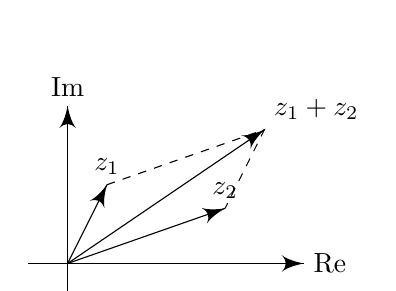
\begin{tikzpicture}
    \draw [->] (-0.5, 0) -- (3, 0) node [right] {Re};
    \draw [->] (0, -0.5) -- (0, 2) node [above] {Im};
    \draw [->] (0, 0) -- (.5, 1) node [above] {$z_1$};
    \draw [->] (0, 0) -- (2, .7) node [above] {$z_2$};
    \draw [->] (0, 0) -- (2.5, 1.7) node [anchor=south west] {$z_1 + z_2$};
    \draw [dashed] (.5, 1) -- (2.5, 1.7) -- (2, .7);
  \end{tikzpicture}
\end{center}

The absolute value of a complex number $x + y i = z \in \C$ is defined by
\[
    |z| = \sqrt{x^2 + y^2}.
\]
Note that $|z| = \norm{(x,y)}= \norm{T(z)}$ where $\norm{\cdot}$ is the standard
Euclidean norm on $\R^2$.

This implies that $|z - w|$ should be considered the distance between natural
numbers $z$, $w$.
Because we have that $|z| = \norm{T(z)}$ we also have that the triangle
inequality holds:
\[
    |z + w| \le |z| + |w| \text{ for all } z,w \in \C.
\]

\begin{definition}[Complex conjugate]
    The complex conjugate of $x + y i = z \in C$ is the complex number
    $x - y i$. The complex conjugate of $z$ is denoted $\bar{z}$.
\end{definition}

\begin{center}
  \begin{tikzpicture}
    \draw [->] (-0.5, 0) -- (3, 0) node [right] {Re};
    \draw [->] (0, -1) -- (0, 2) node [above] {Im};
    \draw [->] (0, 0) -- (2, .7) node [above] {$z_2$};
    \draw [->] (0, 0) -- (2, -.7) node [above] {$\bar z_2$};
  \end{tikzpicture}
\end{center}

It is easy to verify that
\[
    \Re(z) = \frac{z + \bar{z}}{2} \tand 
    \Re(z) = \frac{z - \bar{z}}{2 i} \tand
    |z|^2 = z \bar{z}.
\]

Given $\theta$ we can denote $e^{i \theta} = \cos \theta + i \sin \theta$,
and then describe any complex number $z \in \C$ as $r e^{i \theta}$
for some $\theta \in [0, 2\pi)$ and $r > 0$.
We get that $|z| = |r e^{i \theta}| = r$.
We also have that $\theta$ describes the angle of $z$ with the $x$-axis
and it is usually denoted $\theta = \arg(z)$.

\subsection{Convergence}

\begin{definition}[Convergence]
    We say that the sequence $\set{z_n}_{n \geq 1} \subset \C$ converges
    to some $z_0 \in \C$ if $|z - z_0| \taking{n \to \infty} 0$.
    In this case, we call $z_0$ the limit of the sequence of
    $\set{z_n}_{n \geq 1}$.
\end{definition}

\begin{remark}
    It is easy to verify that the limit is unique, and that
    $z_n \taking{n \to \infty} z$ if and only if
    $T(z_n) \taking{n \to \infty} T(z)$ in the Euclidean metric.
\end{remark}

\begin{definition}[Cauchy sequence]
    A sequence $\set{z_n}_{n \geq 1}$ is said to be a Cauchy sequence if for
    all $\espilon > 0$ there exists $N > 1$ such that for all $n,m > N$
    we have that $|z_n - z_m| < \epsilon$.
\end{definition}

\begin{proposition}
    The complex plane $\C$ is complete.
    That is, every Cauchy sequence converges in $\C$.
\end{proposition}
\begin{proof}
    The proof follows immediately from the known fact that $\R$ is complete
    and the previous remark.
\end{proof}

\subsection{Sets in the complex plane}

\begin{definition}[Open disc]
    For $z_0 \in \C$ and $r > 0$ we set
    \[
        D_r(z_0) := \set{z \in \C \colon |z - z_0| < r}.
    \]
    We call $D_r(z_0)$ the open disc at center $z_0$ with radius $r$.
\end{definition}


\begin{definition}[Closed disc]
    For $z_0 \in \C$ and $r > 0$ we set
    \[
        \overline D_r(z_0) := \set{z \in \C \colon |z - z_0| \le r}.
    \]
    We call $\overline D_r(z_0)$ the closed disc at center $z_0$ with
    radius $r$.
\end{definition}

\begin{definition}[Circle]
    For $z_0 \in \C$ and $r > 0$ we set
    \[
        C_r(z_0) := \set{z \in \C \colon |z - z_0| = r}.
    \]
    We call $C_r(z_0)$ the circle at center $z_0$ with radius $r$.
\end{definition}

\begin{definition}[Interior point]
    Given $\Omega \subset \C$, we say that $z \in \Omega$ is an interior
    point of $\Omega$ if exists $r > 0$ such that $D_r(z) \subset \Omega$.
\end{definition}

\begin{definition}[Interior of a set]
    Given $\Omega \subset \C$, we say that the interior of $\Omega$ is
    the collection of all interior points of $\Omega$.
    We denote the interior as $\Int(\Omega)$.
\end{definition}

\begin{definition}[Open set]
    Given $\Omega \subset \C$, we say that $\Omega$ is an open set if
    $\Int(\Omega) = \Omega$.
\end{definition}

\begin{definition}[Closed set]
    Given $\Omega \subset \C$, we say that $\Omega$ a closed set if
    $\Omega^c := \C \setminus \Omega$ is open.
\end{definition}

\begin{definition}[Limit point]
    Given $\Omega \subset \C$, we say that $z \in \Omega$ is an interior
    point of $\Omega$ if there exists a sequence $z_n$ such that
    $z_n \neq z$ for all $n > 1$ and $z_n \taking{n \to \infty} z$.
\end{definition}

\begin{proposition}
    Let $\Omega \subset \C$ be given.
    Then $\Omega$ is closed if and only if it contains
    all of its limit points.
\end{proposition}
\begin{proof}
    Clear.
\end{proof}

\begin{definition}[Closure]
    Let $\Omega \subset \C$ be given.
    The closure of $\Omega$, denoted $\overline \Omega$, is defined
    as
    \[
        \overline \Omega =
        \Omega \cup
        \set{z \in \C \mid \text{$x$ is a limit point of $\Omega$}}.
    \]
\end{definition}

\begin{remark}
    Note that $\Omega$ is closed if and only if $\overline \Omega = \Omega$.
\end{remark}

\begin{definition}[Boundary]
    The boundary of $\Omega \subset \C$ is denoted by $\partial \Omega$
    and defined by $\partial \Omega := \Omega \setminus \Int(\Omega)$.
\end{definition}

\begin{definition}[Diameter]
    Given $\Omega \subset \C$, we define the diameter of $\Omega$ as
    \[
        \diam(\Omega) := \sup\set{|z - w| \colon z,w \in \Omega}.
    \]
\end{definition}

\begin{definition}[Bounded set]
    Given $\Omega \subset \C$, we say that $\Omega$ is bounded if
    $\diam(\Omega) < \infty$.
\end{definition}

\begin{remark}
    It is clear that a set $\Omega \susbet \C$ is bounded if and only if
    there exists $z_0 \in \C$ and $r > 0$ such that $\Omega \susbet D_r(z_0)$.
\end{remark}

\begin{definition}[Compact set]
    A subset $\Omega$ of $\C$ is said to be compact if it is closed and 
    bounded.
\end{definition}

\begin{theorem}\tt{Bolzano--Weierstrass theorem}
    A subset $\Omega$ in $\C$ is compact if and only if every seqeuence
    $\set{z_n}_{n \geq 1}$ has a subsequence $\set{z_{n_k}}$ such that
    $z_{n_k} \taking{k \to \infty} z$ for some $z \in \C$.
\end{theorem}

\begin{theorem}\tt{Cantor's intersection lemma}
    Let $\Omega_1, \Omega_2, \dots$ be nonempty compact subsets of $\C$.
    Suppose that $\Omega_{n+1} \subset \Omega_n$ for all $n \geq 1$,
    and that $\diam(\Omega_n) \taking{n \to \infty} 0$.
    Then $\cap_{n \geq 1} \Omega_n = \set{z}$ for some $z \in \C$.
\end{theorem}
\begin{proof}
    Choose $z_n \in \Omega_n$ for all $n \geq 1$.
    Because $\diam \Omega \taking{n \to \infty} = 0$ we have that
    $\set{z_n}_{n \geq 1}$ is a Cauchy sequence and therefore it converges
    to some $z \in \C$. Because $\Omega_n$ is compact for every $n \geq 1$
    we get that $z \in \cap_{n \geq 1} \Omega_n$.
    This means that $\cap_{n \geq 1} \Omega_n \neq \emptyset$.

    Let $z,w \in \Omega$.
    Because $\diam \Omega \taking{n \to \infty} 0$ we have that
    $|z - w| \le 0$ and thus $z = w$ which implies that
    $\cap_{n \geq 1} \Omega_n = \set{z}$ which completes the proof.
\end{proof}

\begin{definition}[Connected open set]
    A nonempty open set $\Omega \subset \C$ is said to be connected if it does
    not contain disjoint nonempty open subsets $\Omega_1$, $\Omega_2$ such
    that $\Omega = \Omega_1 \cup \Omega_2$. A connected open set in 
    $\C$ will be called a region.
\end{definition}

\begin{definition}[Connected closed set]
    A nonempty open set $\Omega \subset \C$ is said to be connected if it does
    not contain disjoint nonempty closed subsets $\Omega_1$, $\Omega_2$ such
    that $\Omega = \Omega_1 \cup \Omega_2$.
\end{definition}

\begin{remark}
    It can be shown that $\Omega$ is connected if and only if for any
    $z, w \in \Omega$ there exists a curve $\gamma \colon [0,1] \to \Omega$
    such that $\gamma(0) = z$ and $\gamma(1)$.
    This implies that open and closed discs, as well as circles, are
    connected.
\end{remark}

\subsection{Continuous functions}

\begin{definition}[Continuous function]
    Let $\Omega$ be a nonempty subset of $\C$ and let 
    $f \colon \Omega \to \C$ be given.
    We say that $f$ is continuous at a point $z_0 \in \Omega$ 
    if for all $\epsilon > 0$ there exists $\delta > 0$ so
    that $|f(z) - f(z_0)| < \epsilon$ for all $z \in \Omega$ with 
    $|z - z_0| < \delta$.
    We say that $f$ is continuous on $\Omega$ if it is continuous at every 
    $z_0 \in \Omega$.
\end{definition}

\begin{remark}
    It is easy to verify that the functions $\Im$, $\Re$, $|\cdot|$, and
    $\theta \mapsto e^{i \theta}$ are all continuous.
\end{remark}

\begin{proposition}
    The composition of continuous functions is continuous.
\end{proposition}

\begin{definition}[Bounded function]
    Let $\Omega$ be a nonempty subset of $\C$ and let 
    $f \colon \Omega \to \C$ be given.
    We say that $f$ is bounded if there exists $M > 0$ so that 
    $|f(z)| < M$ for all $z \in \Omega$.
    We say that $f$ attains a maximum if there exists $z_M \in \Omega$
    such that $f(z) \le f(z_M)$ for all $z \in \Omega$.
    We define when $f$ attains a minimum similarly.
\end{definition}

\begin{proposition}
    Let $\Omega$ be a nonempty compact subset of $\C$, and let 
    $f \colon \Omega \to \C$ be continuous.
    Then $f$ is bounded, and it attains its maximum and minimum on $\Omega$.
\end{proposition}

\subsection{Holomorphic functions}

\begin{definition}[Holomorphic function]
    Let $\Omega$ be a nonempty open subset of $\C$ and let 
    $f \colon \Omega \to \C$ be given.
    We say that $f$ is holomorphic at a point $z \in \Omega$
    if the following limit exists
    \[
        f'(z) := \lim_{h \to 0} \frac{f(z + h) - f(z)}{h}.
    \]
    The number $f'(z)$ is called the derivative of $f$ at $z$.
\end{definition}

























\end{document}
